\chapter{Enthalpies de réaction}\label{ch:b2:reaction-enthalpy}

Une cartouche de gaz de camping vissée sous un petit réchaud~: quelques
grammes de butane portent un litre d'eau à ébullition en quelques minutes,
et la flamme bleue sous la casserole est bien plus chaude que l'eau qui
bout. Quelle chaleur une réaction libère-t-elle, quelle part en reçoit la
casserole, et quelle température la flamme peut-elle atteindre~? Aucune de
ces questions n'exige un réchaud pour trouver sa réponse~: des tables de
quelques nombres par substance, mesurés une fois pour toutes, donnent la
chaleur de toute réaction que l'on peut écrire avec ces substances, à
toute température. Ce chapitre construit cette comptabilité. Il applique
le premier principe de la thermodynamique, connu de la physique, à un
système dont la composition change, définit l'\omterm{def:b2:reaction-enthalpy:reaction-quantity}{enthalpie de réaction} comme
une dérivée partielle, et montre comment la calculer à partir des
enthalpies de formation, des enthalpies de liaison ou le long de cycles,
comment elle varie avec la température, et ce qu'elle dit des flammes et
des calorimètres.

\begin{recall}
En physique~: le premier principe $\Delta U = W + Q$~; l'enthalpie $H = U + pV$,
fonction d'état~; à pression extérieure constante, entre deux états à
cette pression, la chaleur reçue est $Q_p = \Delta H$~; la capacité thermique à
pression constante $C_p = (\partial H/\partial T)_p$~; l'enthalpie d'un
gaz parfait ne dépend que de $T$. Le volume de première année a décrit un
système en réaction par son avancement $\xi$ et les nombres stœchiométriques $\nu_i$ de
$0 = \sum_i\nu_i\mathrm A_i$, et fixé l'état standard de chaque espèce
à $p^\circ = \qty{1}{bar}$. Le volume scolaire (année 11) a qualifié une réaction
d'\omterm{def:b2:reaction-enthalpy:exothermic}{exothermique} lorsqu'elle libère de la chaleur, et estimé des énergies de
combustion à partir des énergies de liaison.
\end{recall}

\begin{omfigure}
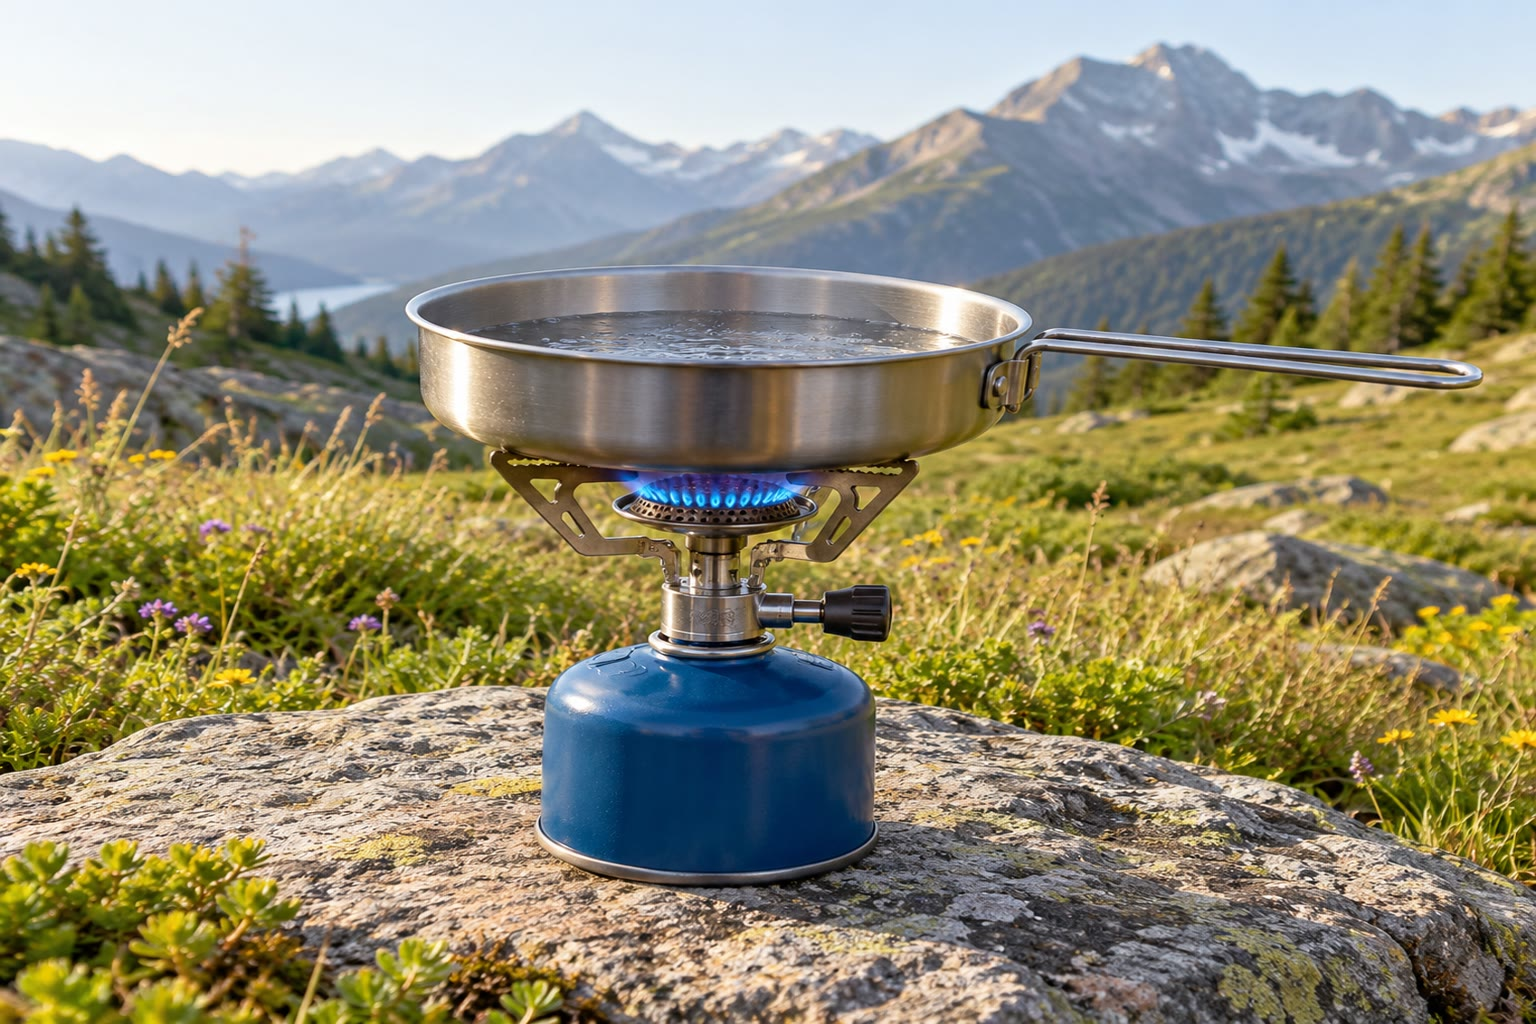
\includegraphics[width=0.6\linewidth]{images/book3/ai/b2-01-camping-stove.jpg}

{\small Un réchaud de camping~: le butane de la cartouche brûle dans l'air sous
la casserole. La chaleur libérée par mole de butane, la part qui atteint
l'eau et la température de la flamme sont calculées dans le problème du
week-end de ce chapitre.}
\end{omfigure}

\section{Grandeurs de réaction}

Un système fermé siège de la seule réaction $0 = \sum_i\nu_i\mathrm A_i$
est décrit par sa température, sa pression et son avancement~:
les quantités sont $n_i = n_{i,0} + \nu_i\xi$. Toute fonction d'état extensive
du système, son enthalpie par exemple, est alors une fonction $H(T, p,
\xi)$, de différentielle totale
\[
  \dd H = \left(\frac{\partial H}{\partial T}\right)_{p,\xi}\dd T
        + \left(\frac{\partial H}{\partial p}\right)_{T,\xi}\dd p
        + \left(\frac{\partial H}{\partial \xi}\right)_{T,p}\dd\xi .
\]

\begin{definition}[Grandeur de réaction, enthalpie de réaction]\label{def:b2:reaction-enthalpy:reaction-quantity}
Pour une fonction d'état extensive $X$ d'un système fermé siège de la
réaction $0 = \sum_i\nu_i\mathrm A_i$, la \emph{grandeur de
réaction}\index{grandeur de reaction@grandeur de réaction} est la dérivée partielle
\[
  \Delta_r X = \left(\frac{\partial X}{\partial \xi}\right)_{T,p} ,
\]
c'est-à-dire la variation de $X$ par unité d'avancement à température et
pression fixées, en unités de $X$ par mole. Pour $X = H$, c'est l'\emph{enthalpie
de réaction}\index{enthalpie de reaction@enthalpie de réaction} $\Delta_r H$, en \unit{kJ/mol}.
\end{definition}

\begin{remark}[Une dérivée, non une différence]\label{rem:b2:reaction-enthalpy:operator}
Le symbole $\Delta_r$ est un opérateur~: il s'applique à un état du
système, qu'il laisse inchangé. Écrire la réaction autrement (doubler ses
coefficients) double $\Delta_r H$~: une \omterm{def:b2:reaction-enthalpy:reaction-quantity}{grandeur de réaction} n'a donc pas
de sens sans son équation. Lorsqu'on utilise les enthalpies molaires partielles
$\bar H_i = (\partial H/\partial n_i)_{T,p,n_j}$ des espèces
(\cref{ch:b2:chemical-potential}), $\Delta_r H = \sum_i\nu_i\bar H_i$, par
dérivation composée de $n_i = n_{i,0} + \nu_i\xi$.
\end{remark}

\begin{proposition}[Chaleur reçue à température et pression constantes]\label{prop:b2:reaction-enthalpy:qp}
Lorsque la réaction avance de $\xi_1$ à $\xi_2$ dans un système maintenu à
$T$ et $p$ constantes, le système reçoit la chaleur
\[
  Q_p = \int_{\xi_1}^{\xi_2}\Delta_r H\,\dd\xi = \Delta_r H\,(\xi_2 - \xi_1)
\]
lorsque $\Delta_r H$ ne dépend pas de $\xi$.
\end{proposition}

\begin{proof}
À $p$ constante (et, ici, à pression extérieure constante), la chaleur reçue
est la variation d'enthalpie, $Q_p = \Delta H$ (physique). À $T$ et $p$ fixées,
la différentielle de $H$ se réduit à $\dd H = \Delta_r H\,\dd\xi$~; l'intégration
de $\xi_1$ à $\xi_2$ donne le résultat.
\end{proof}

\begin{definition}[Exothermique, endothermique, athermique]\label{def:b2:reaction-enthalpy:exothermic}
Une réaction est \emph{exothermique}\index{exothermique} dans un état donné si
$\Delta_r H < 0$~: conduite dans le sens direct à $T$ et $p$ constantes, elle cède de la chaleur au
milieu extérieur. Elle est \emph{endothermique}\index{endothermique} si $\Delta_r H >
0$, et \emph{athermique}\index{athermique} si $\Delta_r H = 0$.
\end{definition}

En général, la chaleur de réaction ne dépend pas de la composition~:
pour des gaz parfaits et pour des solides et des liquides purs, l'enthalpie
de chaque espèce ne dépend pas de ce qui l'entoure, et $\Delta_r H$ est fixée
dès que $T$ l'est.

\begin{proposition}[Systèmes idéaux]\label{prop:b2:reaction-enthalpy:ideal}
Dans un mélange de gaz parfaits et de phases condensées pures, $\Delta_r H$
ne dépend que de la température et est égale à l'\omterm{def:b2:reaction-enthalpy:standard-reaction-enthalpy}{enthalpie standard de
réaction} $\Delta_r H^\circ(T)$ définie plus bas. Pour des solutés en solution
diluée, l'égalité est vraie en bonne approximation.
\end{proposition}

\begin{proof}
Dans un mélange de gaz parfaits, chaque gaz se comporte comme s'il était seul, avec une enthalpie
$n_iH_{m,i}(T)$ qui ne dépend pas de $p$ (physique~: l'enthalpie d'un
gaz parfait ne dépend que de $T$). Un solide ou un liquide pur a pour enthalpie $H = n_iH_{m,i}(T,
p)$, et $(\partial H_m/\partial p)_T = V_m(1 - \alpha T)$ vaut quelques
\unit{J/(mol.bar)} pour une phase condensée, ce qui est négligeable devant des \omterm{def:b2:reaction-enthalpy:reaction-quantity}{enthalpies
de réaction} de plusieurs dizaines de \unit{kJ/mol}. Ainsi $H = \sum_in_iH_{m,i}(T)$, dont la
dérivée par rapport à $\xi$ est $\sum_i\nu_iH_{m,i}(T)$~: elle ne dépend que de
$T$, et sa valeur est celle que l'on calcule avec toutes les espèces dans leur
état standard.
\end{proof}

\section{Enthalpies standard de réaction et loi de Hess}

\begin{definition}[Grandeur standard de réaction]\label{def:b2:reaction-enthalpy:standard-reaction-enthalpy}
La \emph{grandeur standard de réaction}\index{grandeur standard de reaction@grandeur standard de réaction}
$\Delta_r X^\circ(T) = \sum_i\nu_iX_{m,i}^\circ(T)$ est la \omterm{def:b2:reaction-enthalpy:reaction-quantity}{grandeur de réaction}
calculée avec toutes les espèces dans leur état standard à la température $T$, les
$X_{m,i}^\circ$ étant les grandeurs molaires standard. Pour $X = H$, c'est
l'\emph{enthalpie standard de réaction}\index{enthalpie standard de reaction@enthalpie standard de réaction}
$\Delta_r H^\circ(T)$~; elle ne dépend que de $T$.
\end{definition}

Seules les différences d'enthalpie sont mesurables~: on choisit donc une
référence une fois pour toutes, comme on a choisi l'électrode à hydrogène pour les potentiels.

\begin{definition}[État standard de référence, enthalpie standard de formation]\label{def:b2:reaction-enthalpy:formation}
L'\emph{état standard de référence}\index{etat standard de reference@état standard de référence} d'un
élément à la température $T$ est sa forme la plus stable à $T$ sous $p^\circ$~:
\ce{H2}, \ce{O2}, \ce{N2} et \ce{Cl2} en gaz parfaits, le carbone en
graphite, le sodium en métal, le brome en liquide (à \qty{298}{K}).
L'\emph{enthalpie standard de formation}\index{enthalpie standard de formation}
$\Delta_f H^\circ$ d'un composé est l'enthalpie standard de
sa réaction de formation, celle qui produit une mole du
composé à partir de ses éléments dans leur état de référence. Par construction,
$\Delta_f H^\circ = 0$ pour un élément dans son état de référence.
\end{definition}

\begin{example}[Réactions de formation]\label{ex:b2:reaction-enthalpy:formation}
La réaction de formation de l'eau est \ce{H2(g) + 1/2O2(g) -> H2O(l)}, avec
$\Delta_f H^\circ = \qty{-285.83}{kJ/mol}$ à \qty{298.15}{K}~; celle du
méthane est \ce{C(s) + 2H2(g) -> CH4(g)}, $\Delta_f H^\circ =
\qty{-74.9}{kJ/mol}$~; celle du monoxyde d'azote, \ce{1/2N2(g) + 1/2O2(g) ->
NO(g)}, $\Delta_f H^\circ = \qty{+90.3}{kJ/mol}$~: un composé \omterm{def:b2:reaction-enthalpy:exothermic}{endothermique},
que les gaz chauds d'un moteur produisent pourtant. Les coefficients
demi-entiers ne posent pas de problème~: la réaction de formation est un
outil de comptabilité, non un mécanisme.
% ledger: dfh:H2O-l, dfh:CH4_g, dfh:NO_g
\end{example}

\begin{theorem}[Loi de Hess]\label{thm:b2:reaction-enthalpy:hess}
Si une réaction est la somme, avec les coefficients $\lambda_k$, de réactions $k$,
son \omterm{def:b2:reaction-enthalpy:standard-reaction-enthalpy}{enthalpie standard de réaction} est la même combinaison des leurs~:
$\Delta_r H^\circ = \sum_k\lambda_k\Delta_r H_k^\circ$
(\emph{loi de Hess}\index{loi de Hess}). En particulier, une \omterm{def:b2:reaction-enthalpy:standard-reaction-enthalpy}{enthalpie standard de réaction}
peut se calculer le long de tout chemin de réactions qui mène des
réactifs aux produits.
\end{theorem}

\begin{proof}
Chaque $\Delta_r H_k^\circ = \sum_i\nu_{i,k}H_{m,i}^\circ$ est linéaire en les
nombres stœchiométriques. Si la réaction est égale à $\sum_k\lambda_k$ fois les
réactions $k$, ses nombres stœchiométriques sont $\nu_i = \sum_k\lambda_k
\nu_{i,k}$, et $\Delta_r H^\circ = \sum_i\nu_iH_{m,i}^\circ = \sum_k\lambda_k
\sum_i\nu_{i,k}H_{m,i}^\circ$. Derrière l'algèbre se trouve le premier principe~: $H$ est une
fonction d'état, sa variation entre les mêmes états initial et final
ne dépend donc pas du chemin suivi.
\end{proof}

\begin{proposition}[Enthalpie de réaction à partir des enthalpies de formation]\label{prop:b2:reaction-enthalpy:formation-sum}
$\Delta_r H^\circ(T) = \sum_i\nu_i\,\Delta_f H_i^\circ(T)$.
\end{proposition}

\begin{proof}
Prendre le chemin qui décompose les réactifs en leurs éléments dans leur
état de référence (l'inverse de leurs réactions de formation, avec les
coefficients $-\nu_i > 0$), puis forme les produits à partir des mêmes éléments
(coefficients $\nu_i > 0$). Les éléments se compensent parce que l'équation est
équilibrée, et la \omterm{thm:b2:reaction-enthalpy:hess}{loi de Hess} additionne les enthalpies.
\end{proof}

\begin{omfigure}
\begin{tikzpicture}[font=\small, >={Stealth}, y=0.0062cm]
  \draw[->] (0,-1000) -- (0,180) node[above] {$H^\circ$ (\unit{kJ/mol})};
  \foreach \y in {0,-200,-400,-600,-800,-1000} \draw (-0.08,\y) -- (0.08,\y) node[left=4pt] {$\y$};
  % levels
  \draw[very thick] (1.0,0) -- (4.6,0) node[right] {\ce{C(s) + 2H2(g) + 2O2(g)}};
  \draw[very thick, omDef] (1.0,-74.9) -- (4.6,-74.9);
  \node[right, omDef] at (4.6,-110) {\ce{CH4(g) + 2O2(g)}};
  \draw[very thick, omThm] (1.0,-965.2) -- (4.6,-965.2) node[right] {\ce{CO2(g) + 2H2O(l)}};
  % arrows
  \draw[->, omDef, thick] (1.6,0) -- (1.6,-74.9);
  \node[omDef, anchor=south west, font=\footnotesize] at (1.1,5) {$\Delta_f H^\circ(\ce{CH4}) = -74.9$};
  \draw[->, omThm, thick] (3.9,0) -- (3.9,-965.2);
  \node[right, omThm, align=left] at (3.95,-500) {$\Delta_f H^\circ(\ce{CO2})$\\ $+ 2\Delta_f H^\circ(\ce{H2O})$\\ $= -965.2$};
  \draw[->, thick] (2.75,-74.9) -- (2.75,-965.2);
  \node[left, align=right] at (2.7,-650) {$\Delta_r H^\circ$\\ $= -890.3$};
\end{tikzpicture}

{\small Niveaux d'enthalpie pour la combustion du méthane à \qty{298.15}{K}.
Les éléments dans leur état de référence sont le zéro. Le méthane se trouve
\qty{74.9}{kJ/mol} au-dessous, les produits \qty{965.2}{kJ/mol} au-dessous~:
l'enthalpie de combustion est la différence, \qty{-890.3}{kJ/mol}, quel que soit
le chemin réellement suivi par la flamme.}
% ledger: dfh:CH4_g, dfh:CO2, dfh:H2O-l
\end{omfigure}

\begin{example}[Combustion du méthane]\label{ex:b2:reaction-enthalpy:methane}
Pour \ce{CH4(g) + 2O2(g) -> CO2(g) + 2H2O(l)},
$\Delta_r H^\circ = -393.51 + 2(-285.83) - (-74.87) - 0 =
\qty{-890.3}{kJ/mol}$ à \qty{298.15}{K}. La valeur mesurée dans un
calorimètre est \qty{-890.7}{kJ/mol}~: la table et la flamme s'accordent à
l'incertitude des données près. Si l'eau sort sous forme de vapeur
($\Delta_f H^\circ = \qty{-241.83}{kJ/mol}$), $\Delta_r H^\circ =
\qty{-802.3}{kJ/mol}$~: la différence, \qty{88.0}{kJ}, est l'enthalpie de
vaporisation de deux moles d'eau, que récupère une chaudière à condensation
en condensant ses fumées.
% ledger: dfh:CO2, dfh:H2O-l, dfh:CH4_g, dch:CH4, dfh:H2O_g (computed in figdata/bachelor-2/thermo-data.py)
\end{example}

\begin{method}[Un cycle de Hess]\label{met:b2:reaction-enthalpy:hess-cycle}
Pour trouver l'enthalpie d'une réaction que l'on ne peut pas mesurer directement~:
\begin{enumerate}
  \item écrire la réaction cible avec les états physiques~;
  \item trouver des réactions d'enthalpie connue (combustions, formations) dont la
        combinaison, avec des coefficients $\lambda_k$, donne la cible~;
  \item vérifier que toute espèce absente de la cible se simplifie~;
  \item additionner les enthalpies avec les mêmes coefficients.
\end{enumerate}
\end{method}

\begin{example}[Du carbone au monoxyde de carbone]\label{ex:b2:reaction-enthalpy:co}
Brûler du carbone produit toujours un peu de dioxyde de carbone~: l'enthalpie de
\ce{C(s) + 1/2O2(g) -> CO(g)} ne se mesure donc pas directement. Les deux combustions
\ce{C(s) + O2(g) -> CO2(g)} ($\qty{-393.51}{kJ/mol}$) et \ce{CO(g) +
1/2O2(g) -> CO2(g)} ($\qty{-283.0}{kJ/mol}$, mesurée), elles, se mesurent~; la cible est
la première moins la seconde~: $\Delta_r H^\circ = -393.51 + 283.0 =
\qty{-110.5}{kJ/mol}$, l'enthalpie de formation du monoxyde de carbone.
% ledger: dfh:CO2, dfh:CO_g
\end{example}

\begin{history}[Germain Henri Hess]
\begin{minipage}[t]{0.2\linewidth}\vspace{0pt}
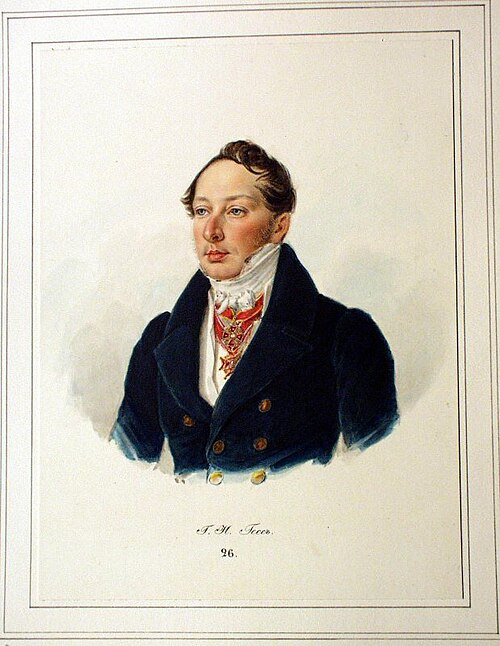
\includegraphics[width=\linewidth]{images/book3/hess.jpg}
\end{minipage}\hfill
\begin{minipage}[t]{0.76\linewidth}\vspace{0pt}
Germain Henri Hess (1802--1850), professeur de chimie à
Saint-Pétersbourg, mesura les chaleurs libérées lorsqu'on dilue ou
neutralise l'acide sulfurique en plusieurs étapes, et constata en 1840 que le total ne
dépendait pas des étapes suivies~: la «~loi de la somme constante des chaleurs~», énoncée
avant le premier principe de la thermodynamique lui-même, qui l'explique.
(Portrait par I. I. Reimers, 1837--1838~; CC BY-SA 4.0, Wikimedia Commons.)
\end{minipage}
\end{history}

\section{Calculer une enthalpie de réaction}

\subsection*{À partir des enthalpies de liaison}

Lorsque l'enthalpie de formation d'un composé manque, l'énergie de ses
liaisons en donne une estimation, en phase gazeuse.

\begin{definition}[Enthalpie de dissociation de liaison, enthalpie moyenne de liaison]\label{def:b2:reaction-enthalpy:bond-enthalpy}
L'\emph{enthalpie de dissociation de liaison}\index{enthalpie de dissociation de liaison} d'une
liaison A--B dans une molécule gazeuse est l'enthalpie standard de la
réaction de rupture de cette liaison en deux fragments gazeux, \ce{AB(g) -> A(g) + B(g)}
pour une molécule diatomique. Lorsqu'une molécule possède $n$ liaisons identiques, son
\emph{enthalpie moyenne de liaison}\index{enthalpie moyenne de liaison} est l'enthalpie
standard de son atomisation complète en atomes gazeux, divisée par $n$.
\end{definition}

Les enthalpies d'atomisation sont elles-mêmes des enthalpies de formation~: celles des
atomes gazeux, moins celle de la molécule. La table ci-dessous est
calculée de cette façon.

\begin{omfigure}
\begin{tabular}{lrl}
\hline
liaison & enthalpie (\unit{kJ/mol}) & obtenue à partir de \\
\hline
H--H & 436 & \ce{H2}, dissociation \\
O=O & 498 & \ce{O2}, dissociation \\
N$\equiv$N & 945 & \ce{N2}, dissociation \\
Cl--Cl & 243 & \ce{Cl2}, dissociation \\
H--Cl & 432 & \ce{HCl}, dissociation \\
C--H & 416 & \ce{CH4}, moyenne sur quatre \\
N--H & 391 & \ce{NH3}, moyenne sur trois \\
O--H & 464 & \ce{H2O}, moyenne sur deux \\
C=O & 804 & \ce{CO2}, moyenne sur deux \\
C--C & 330 & \ce{C2H6}, avec C--H tiré du méthane \\
C=C & 589 & \ce{C2H4}, avec C--H tiré du méthane \\
\hline
\end{tabular}

\smallskip
{\small Enthalpies de liaison à \qty{298.15}{K}, calculées à partir des
\omterm{def:b2:reaction-enthalpy:formation}{enthalpies standard de formation} des atomes et des molécules gazeux. Les deux
dernières lignes montrent la limite de la méthode~: une liaison C--H de l'éthane
n'est pas exactement celle du méthane, et la valeur C--C hérite de l'écart.}
% ledger: dfh:C_g, janaf:H, dfh:O_g, dfh:N_g, janaf:Cl, janaf:HCl, dfh:CH4_g, dfh:NH3_g, dfh:H2O_g, dfh:CO2, dfh:C2H6_g, dfh:C2H4_g (computed in figdata/bachelor-2/thermo-data.py)
\end{omfigure}

\begin{proposition}[Estimation par les enthalpies de liaison]\label{prop:b2:reaction-enthalpy:bond-estimate}
Pour une réaction entre gaz,
\[
  \Delta_r H^\circ \approx \sum(\text{enthalpies des liaisons rompues}) -
  \sum(\text{enthalpies des liaisons formées}).
\]
\end{proposition}

\begin{proof}
Suivre le chemin qui atomise tous les réactifs (enthalpie~: les liaisons rompues),
puis construit les produits à partir des atomes (moins les liaisons formées). La \omterm{thm:b2:reaction-enthalpy:hess}{loi
de Hess} rend la somme exacte lorsque chaque enthalpie de liaison est celle de la liaison dans sa
propre molécule~; la remplacer par une valeur moyenne tirée d'une autre molécule constitue
l'approximation.
\end{proof}

\begin{example}[Hydrogénation de l'éthène]\label{ex:b2:reaction-enthalpy:hydrogenation}
Dans \ce{C2H4(g) + H2(g) -> C2H6(g)}, une C=C et une H--H sont rompues et
remplacées par une C--C et deux C--H. Avec la table~: $589 + 436 - 330 - 2
\times 416 = \qty{-137}{kJ/mol}$~; à partir des enthalpies de formation, la valeur est
\qty{-136.3}{kJ/mol}. L'accord est bon ici parce que les valeurs C--C
et C=C de la table ont été obtenues à partir de ces molécules mêmes~; pour une molécule
différente de celles de la table, une erreur de 10 à \qty{30}{kJ/mol} est courante.
% ledger: dfh:C2H4_g, dfh:C2H6_g
\end{example}

\subsection*{Enthalpies réticulaires~: le cycle de Born--Haber}

\begin{definition}[Enthalpie réticulaire]\label{def:b2:reaction-enthalpy:lattice-enthalpy}
L'\emph{enthalpie réticulaire}\index{enthalpie reticulaire@enthalpie réticulaire} d'un cristal ionique est
l'enthalpie standard de la réaction de sa dissociation en ions gazeux~: pour le
chlorure de sodium, \ce{NaCl(s) -> Na+(g) + Cl-(g)}. Elle est positive et
mesure la cohésion du cristal.
\end{definition}

On ne peut pas la mesurer directement, mais un cycle passant par les éléments la donne
à partir de grandeurs mesurables~: l'enthalpie de formation du cristal,
l'atomisation des éléments, l'énergie d'ionisation du métal et
l'affinité électronique du non-métal (toutes deux définies dans le volume de première année).

\begin{omfigure}
\begin{tikzpicture}[font=\small, >={Stealth}, y=0.0058cm]
  \def\lw{5.0}
  % levels (kJ/mol relative to Na(s) + 1/2 Cl2(g))
  \draw[thick] (0,0) -- (\lw,0) node[right] {\ce{Na(s) + 1/2Cl2(g)}};
  \draw[thick] (0,107.5) -- (\lw,107.5) node[right] {\ce{Na(g) + 1/2Cl2(g)}};
  \draw[thick] (0,228.8) -- (\lw,228.8) node[right] {\ce{Na(g) + Cl(g)}};
  \draw[thick] (0,724.6) -- (\lw,724.6) node[right] {\ce{Na+(g) + e- + Cl(g)}};
  \draw[thick] (0,376.1) -- (\lw,376.1) node[right] {\ce{Na+(g) + Cl-(g)}};
  \draw[thick] (0,-411.1) -- (\lw,-411.1) node[right] {\ce{NaCl(s)}};
  % the path through the elements, on the left
  \draw[->, omDef] (0.4,0) -- (0.4,107.5);
  \node[omDef, left, font=\footnotesize] at (0.35,53) {sublimation $107.5$};
  \draw[->, omDef] (0.4,107.5) -- (0.4,228.8);
  \node[omDef, left, font=\footnotesize] at (0.35,168) {$\tfrac12$ dissociation $121.3$};
  \draw[->, omDef] (0.4,228.8) -- (0.4,724.6);
  \node[omDef, left, font=\footnotesize] at (0.35,480) {ionisation de Na $495.8$};
  \draw[->, omThm] (1.4,724.6) -- (1.4,376.1);
  \node[omThm, right, font=\footnotesize] at (1.45,560) {attachement électronique $-348.6$};
  \draw[->, omProp] (2.3,0) -- (2.3,-411.1);
  \node[omProp, left, font=\footnotesize] at (2.25,-205) {formation $-411.1$};
  % the lattice enthalpy, the only unknown
  \draw[->, thick] (3.6,-411.1) -- (3.6,376.1);
  \node[right, font=\footnotesize] at (3.65,-205) {enthalpie réticulaire $787$};
\end{tikzpicture}

{\small Le cycle de Born--Haber du chlorure de sodium à \qty{298}{K}
(\unit{kJ/mol}). Monter du cristal aux ions gazeux par l'\omterm{def:b2:reaction-enthalpy:lattice-enthalpy}{enthalpie
réticulaire}, ou faire le tour par les éléments, conduit au même niveau~:
l'\omterm{def:b2:reaction-enthalpy:lattice-enthalpy}{enthalpie réticulaire} est la seule inconnue du cycle.}
% ledger: dfh:NaCl_cr, dfh:Na_g, janaf:Cl, ie:Na, ea:Cl
\end{omfigure}

\begin{method}[Le cycle de Born--Haber]\label{met:b2:reaction-enthalpy:born-haber}
\begin{enumerate}
  \item À partir des éléments dans leur état de référence, tracer deux chemins~: l'un
        vers le cristal (formation), l'autre vers les ions gazeux (sublimation du
        métal, atomisation du non-métal, ionisation, attachement
        électronique).
  \item Fermer le cycle par l'\omterm{def:b2:reaction-enthalpy:lattice-enthalpy}{enthalpie réticulaire}, du cristal jusqu'aux
        ions gazeux.
  \item Écrire que la somme des enthalpies sur le cycle est nulle, et
        en tirer l'inconnue. Les énergies d'ionisation et les affinités électroniques
        sont tabulées en eV par atome~: multiplier par $N_A e = \qty{96.485}{kJ/(mol.eV)}$.
\end{enumerate}
\end{method}

\begin{example}[Le chlorure de sodium]\label{ex:b2:reaction-enthalpy:nacl}
$\Delta_{\text{rét}}H^\circ = 411.1 + 107.5 + 121.3 + 495.8 - 348.6 =
\qty{787}{kJ/mol}$. L'énergie d'ionisation et l'affinité électronique sont
des énergies à \qty{0}{K}~; leurs corrections à \qty{298}{K} ($+\tfrac52RT$
pour chacune) se compensent entre les deux étapes. Un modèle de cristal à charges ponctuelles
donne une valeur voisine~: c'est pourquoi on qualifie le chlorure de sodium d'ionique.
% ledger: dfh:NaCl_cr, dfh:Na_g, janaf:Cl, ie:Na, ea:Cl (computed in figdata/bachelor-2/thermo-data.py)
\end{example}

\section{Enthalpies de réaction et température}

Les tables donnent $\Delta_f H^\circ$ à \qty{298.15}{K}. Un réacteur fonctionne à
\qty{700}{K}, une flamme à \qty{2000}{K}~: comment $\Delta_r H^\circ$ varie-t-elle
avec la température~?

\begin{theorem}[Loi de Kirchhoff]\label{thm:b2:reaction-enthalpy:kirchhoff}
\[
  \frac{\dd\Delta_r H^\circ}{\dd T} = \Delta_r C_p^\circ =
  \sum_i\nu_i C_{p,m,i}^\circ ,
\]
de sorte que $\Delta_r H^\circ(T_2) = \Delta_r H^\circ(T_1) + \int_{T_1}^{T_2}
\Delta_r C_p^\circ\,\dd T$ (\emph{loi de Kirchhoff}\index{loi de Kirchhoff}),
en l'absence de changement d'état entre $T_1$ et $T_2$.
\end{theorem}

\begin{proof}
Toutes les espèces étant dans leur état standard, $H^\circ(T, \xi) = \sum_in_i
H^\circ_{m,i}(T)$ est une fonction de deux variables dont les dérivées partielles
secondes sont continues~; d'après le théorème de Schwarz, elles commutent~:
\[
  \frac{\dd\Delta_r H^\circ}{\dd T} = \frac{\partial}{\partial T}
  \frac{\partial H^\circ}{\partial\xi} = \frac{\partial}{\partial\xi}
  \frac{\partial H^\circ}{\partial T} = \frac{\partial}{\partial\xi}
  \sum_in_iC^\circ_{p,m,i} = \sum_i\nu_iC^\circ_{p,m,i}.
\]
L'intégration entre $T_1$ et $T_2$ donne la seconde forme. Un changement
d'état d'une espèce à l'intérieur de l'intervalle ajoute son enthalpie de
changement d'état, affectée du nombre stœchiométrique.
\end{proof}

\begin{example}[La synthèse de l'ammoniac à chaud]\label{ex:b2:reaction-enthalpy:kirchhoff}
Pour \ce{N2(g) + 3H2(g) -> 2NH3(g)}, $\Delta_r H^\circ(298) =
\qty{-91.9}{kJ/mol}$ et, avec les capacités thermiques à \qty{298}{K},
$\Delta_r C_p^\circ = 2(35.65) - 29.12 - 3(28.84) =
\qty{-44.3}{J/(K.mol)}$. Supposée constante, elle donne $\Delta_r
H^\circ(700) = -91.9 - 0.0443 \times 402 = \qty{-109.7}{kJ/mol}$. Les tables,
qui suivent la croissance des capacités thermiques avec la température, donnent
\qty{-105.2}{kJ/mol}~: l'estimation à $C_p$ constante est en erreur de 4\,\%, un
prix raisonnable pour un calcul d'une ligne. Sur \qty{400}{K}, l'\omterm{def:b2:reaction-enthalpy:reaction-quantity}{enthalpie de
réaction} varie d'environ un septième.
% ledger: dfh:NH3_g, cp:NH3_g.298, cp:N2_g.298, cp:H2_g.298, janafdfH:NH3.700 (computed in figdata/bachelor-2/thermo-data.py)
\end{example}

\section{Réactions adiabatiques et calorimétrie}

\subsection*{Température de flamme}

Dans une flamme, la réaction est rapide et la chaleur n'a pas le temps de s'échapper~: les
gaz s'échauffent eux-mêmes.

\begin{definition}[Température de flamme adiabatique]\label{def:b2:reaction-enthalpy:flame-temperature}
La \emph{température de flamme adiabatique}\index{temperature de flamme adiabatique@température de flamme adiabatique}
d'un combustible est la température atteinte par les produits de sa combustion
complète lorsque la réaction a lieu à pression constante, sans
aucun échange de chaleur, à partir de réactifs à \qty{298}{K}.
\end{definition}

\begin{proposition}[Calcul d'une température de flamme]\label{prop:b2:reaction-enthalpy:flame}
Si la réaction avance de $\xi$ à partir de réactifs à $T_0$ et si le système final
a pour capacité thermique $C_p(T)$, la température finale $T_f$ vérifie
\[
  \xi\,\Delta_r H^\circ(T_0) + \int_{T_0}^{T_f}C_p(T)\,\dd T = 0 .
\]
\end{proposition}

\begin{proof}
Adiabatique et à pression constante, la transformation vérifie $\Delta H =
Q_p = 0$. Comme $H$ est une fonction d'état, tout chemin entre les mêmes états initial et
final donne la même $\Delta H$. Prenons le chemin de
la figure ci-dessous~: d'abord la réaction à $T_0$, avec
$\Delta H_1 = \xi\Delta_r H^\circ(T_0)$ (\cref{prop:b2:reaction-enthalpy:qp},
dans l'hypothèse d'un comportement idéal)~; puis l'échauffement du système final de $T_0$ à
$T_f$, $\Delta H_2 = \int C_p\,\dd T$. Leur somme est nulle.
\end{proof}

\begin{omfigure}
\begin{tikzpicture}[font=\small, >={Stealth}]
  \draw[->] (0,0) -- (6.2,0) node[right] {avancement $\xi$};
  \draw[->] (0,0) -- (0,3.6) node[above] {température $T$};
  \fill (0.6,0.6) circle (2pt) node[below left] {réactifs, $T_0$};
  \fill (5.2,0.6) circle (2pt) node[below] {produits, $T_0$};
  \fill (5.2,3.0) circle (2pt) node[right] {produits, $T_f$};
  \draw[->, thick, omDef] (0.7,0.6) -- (5.1,0.6);
  \node[omDef, above, font=\footnotesize] at (3.15,0.64) {$\Delta H_1 = \xi\,\Delta_r H^\circ(T_0) < 0$};
  \draw[->, thick, omThm] (5.2,0.7) -- (5.2,2.9);
  \node[omThm, right, align=left] at (5.25,1.8) {$\Delta H_2 = \int_{T_0}^{T_f} C_p\,\dd T$};
  \draw[->, thick, dashed] (0.75,0.75) -- (5.05,2.92);
  \node[above left, align=center] at (2.6,1.75) {flamme réelle~:\\ $\Delta H = 0$};
\end{tikzpicture}

{\small La flamme adiabatique (en tirets) et un chemin équivalent en deux
étapes~: réaction à température constante, puis échauffement des produits.
$H$ étant une fonction d'état, les deux variations d'enthalpie des étapes ont
une somme nulle.}
\end{omfigure}

\begin{method}[Température de flamme]\label{met:b2:reaction-enthalpy:flame-temperature}
\begin{enumerate}
  \item Écrire la combustion complète d'une mole de combustible~; dans l'air, ajouter
        le diazote et l'argon qui accompagnent le dioxygène (ils sont chauffés
        eux aussi)~; prendre l'eau à l'état de vapeur.
  \item Calculer $q = -\Delta_r H^\circ(T_0)$ par mole de combustible.
  \item Soit prendre une capacité thermique $C_p$ des produits constante~:
        $T_f = T_0 + q/C_p$~; soit chercher par interpolation la $T_f$ telle que la somme des
        incréments tabulés $n_i[H^\circ_{m,i}(T_f) - H^\circ_{m,i}(T_0)]$
        soit égale à $q$.
\end{enumerate}
\end{method}

\begin{omfigure}
\begin{tikzpicture}
\begin{axis}[
  width=0.8\linewidth, height=6.2cm, xmin=300, xmax=3000, ymin=0, ymax=3200,
  axis x line=bottom, axis y line=left, xlabel={$T$ (K)},
  ylabel={$H(T) - H(\qty{298}{K})$ des produits (kJ)},
  xtick={500,1000,1500,2000,2500,3000},
  tick label style={font=\small}, label style={font=\small}, clip=false,
  legend style={font=\scriptsize, draw=none, at={(0.5,1.03)}, anchor=south}, legend columns=2]
\addplot[omDef, very thick] table[x=T, y=H] {figdata/out/bachelor-2-flame-temperature-butane.dat};
\addplot[omThm, very thick] table[x=T, y=H] {figdata/out/bachelor-2-flame-temperature-methane.dat};
\legend{1 mol de butane dans l'air, 1 mol de méthane dans l'air}
\draw[omDef, dashed] (axis cs:300,2657.6) -- (axis cs:3000,2657.6);
\node[omDef, anchor=south east, font=\scriptsize] at (axis cs:2350,2657.6) {$-\Delta_r H^\circ = \qty{2657.6}{kJ}$};
\draw[omDef, dotted] (axis cs:2401,0) -- (axis cs:2401,2657.6);
\fill[omDef] (axis cs:2401,2657.6) circle (1.5pt);
\node[omDef, anchor=north west, font=\scriptsize] at (axis cs:2420,2620) {\qty{2401}{K}};
\draw[omThm, dashed] (axis cs:300,802.3) -- (axis cs:3000,802.3);
\node[omThm, anchor=south west, font=\scriptsize] at (axis cs:320,802.3) {$-\Delta_r H^\circ = \qty{802.3}{kJ}$};
\draw[omThm, dotted] (axis cs:2329,0) -- (axis cs:2329,802.3);
\fill[omThm] (axis cs:2329,802.3) circle (1.5pt);
\node[omThm, anchor=north west, font=\scriptsize] at (axis cs:2350,760) {\qty{2329}{K}};
\end{axis}
\end{tikzpicture}

{\small Enthalpie nécessaire pour chauffer à partir de \qty{298}{K} les produits de combustion d'une
mole de combustible (dioxyde de carbone, vapeur d'eau, diazote et argon de
l'air), d'après les enthalpies tabulées. Chaque courbe rencontre la chaleur
libérée par sa combustion à la \omterm{def:b2:reaction-enthalpy:flame-temperature}{température de flamme adiabatique}~: environ
\qty{2400}{K} pour le butane, \qty{2330}{K} pour le méthane.}
% ledger: janafH:CO2.2400, janafH:H2O.2400, janafH:N2.2400, janafH:Ar.2400, air:N2, air:O2, air:Ar (computed in figdata/bachelor-2/flame-temperature.py)
\end{omfigure}

Les températures calculées sont des bornes supérieures. Au-dessus d'environ \qty{2000}{K},
le dioxyde de carbone et l'eau commencent à se dissocier en monoxyde de carbone,
dihydrogène, dioxygène et radicaux~; ces réactions \omterm{def:b2:reaction-enthalpy:exothermic}{endothermiques} reprennent une partie
de la chaleur, et une flamme réelle de butane dans l'air est sensiblement plus froide
que le calcul ne l'indique. Dans le dioxygène pur, il n'y a pas de diazote à chauffer et la flamme est
bien plus chaude~: c'est pourquoi les soudeurs brûlent l'éthyne avec du dioxygène plutôt qu'avec
de l'air.

\subsection*{Calorimétrie}

\begin{proposition}[Volume constant et pression constante]\label{prop:b2:reaction-enthalpy:bomb}
Dans une enceinte close en acier (une bombe calorimétrique), la chaleur mesurée est $Q_V =
\Delta U$, et pour des gaz parfaits et des phases condensées
\[
  \Delta_r H = \Delta_r U + \Delta\nu_{\text{gaz}}\,RT ,
\]
où $\Delta\nu_{\text{gaz}}$ est la somme des nombres stœchiométriques des
espèces gazeuses.
\end{proposition}

\begin{proof}
$H = U + pV$, et $\Delta_r H = \Delta_r U + \partial(pV)/\partial\xi$ à
$T$ fixée. Le produit $pV$ des phases condensées est négligeable, et pour les
gaz $pV = n_{\text{gaz}}RT$ avec $n_{\text{gaz}} = n_{\text{gaz},0} +
\Delta\nu_{\text{gaz}}\xi$, dont la dérivée par rapport à $\xi$ est
$\Delta\nu_{\text{gaz}}RT$.
\end{proof}

\begin{omfigure}
\begin{tikzpicture}[font=\small, >={Stealth}, scale=1.0]
  % outer insulated jacket
  \draw[thick, fill=gray!8] (-2.6,-0.2) rectangle (2.6,4.4);
  \draw[thick, fill=white] (-2.3,0.1) rectangle (2.3,4.1);
  % water bath
  \fill[omDef!12] (-2.3,0.1) rectangle (2.3,3.4);
  \draw[omDef!60] (-2.3,3.4) -- (2.3,3.4);
  % bomb
  \draw[very thick, fill=gray!35] (-0.75,0.5) rectangle (0.75,2.6);
  \draw[very thick, fill=gray!55] (-0.9,2.6) rectangle (0.9,2.85);
  \draw[thick] (-0.3,1.0) -- (-0.3,1.9) (0.3,1.0) -- (0.3,1.9);
  \draw[thick, fill=orange!50] (-0.3,0.95) rectangle (0.3,1.05);
  \draw[red!70!black, thick, decorate, decoration={zigzag, amplitude=1pt, segment length=3pt}] (-0.3,1.9) -- (0.3,1.9);
  % wires
  \draw (-0.3,2.85) -- (-0.3,4.7) (0.3,2.85) -- (0.3,4.7);
  % stirrer and thermometer
  \draw[thick] (1.6,0.6) -- (1.6,4.7);
  \draw[thick, fill=gray!40] (1.35,0.55) rectangle (1.85,0.75);
  \pic[transform shape] at (-1.6,0.4) {thermometer};
  % labels
  \draw (-0.75,1.6) -- (-3.3,1.6) node[left] {bombe en acier, \ce{O2} à 30 bar};
  \draw (0,1.0) -- (-3.3,0.6) node[left] {échantillon dans sa coupelle};
  \draw (0,1.9) -- (-3.3,2.6) node[left] {fil d'allumage};
  \draw (1.0,3.0) -- (3.3,3.0) node[right] {bain d'eau};
  \draw (1.6,3.9) -- (3.3,4.3) node[right] {agitateur};
  \draw (-1.6,3.4) -- (-3.3,3.6) node[left] {thermomètre};
  \draw (2.45,0.3) -- (3.3,0.5) node[right] {enveloppe isolante};
\end{tikzpicture}

{\small Une bombe calorimétrique. L'échantillon brûle à volume constant dans
le dioxygène sous pression~; la chaleur passe dans la bombe et dans l'eau agitée,
dont on lit l'élévation de température sur le thermomètre. La capacité
thermique du calorimètre est déterminée au préalable en brûlant un étalon d'énergie connue.}
\end{omfigure}

\begin{method}[Calorimétrie]\label{met:b2:reaction-enthalpy:calorimetry}
\begin{enumerate}
  \item Étalonner~: brûler une masse d'un étalon d'énergie de combustion connue
        (ou fournir une énergie électrique connue), lire l'élévation de température
        $\Delta T$, et en déduire la capacité thermique $C$ de l'ensemble du
        calorimètre (eau et récipient, sa «~valeur en eau~»).
  \item Brûler l'échantillon, lire $\Delta T'$~: la chaleur libérée est $C\,\Delta
        T'$, d'où $\Delta_r U = -C\Delta T'/\xi$ à volume constant.
  \item Corriger pour obtenir $\Delta_r H$ avec $\Delta\nu_{\text{gaz}}RT$~; dans un calorimètre
        ouvert (à pression constante), $\Delta_r H = -C\Delta T'/\xi$
        directement.
\end{enumerate}
\end{method}

\begin{example}[Une mesure à la bombe]\label{ex:b2:reaction-enthalpy:bomb}
Pour la combustion du butane avec formation d'eau liquide, $\Delta\nu_{\text{gaz}} = 4
- 1 - 6.5 = -3.5$, donc $\Delta_r U = \Delta_r H + 3.5RT = -2877.6 + 8.7 =
\qty{-2868.9}{kJ/mol}$~: la correction est de quelques millièmes, plus grande
que l'incertitude d'une bonne mesure à la bombe~; on ne l'omet donc jamais.
% ledger: dfh:C4H10_g, dfh:CO2, dfh:H2O-l (computed in figdata/bachelor-2/thermo-data.py)
\end{example}

\begin{history}[Les bombes calorimétriques, 1881]
\begin{minipage}[t]{0.2\linewidth}\vspace{0pt}
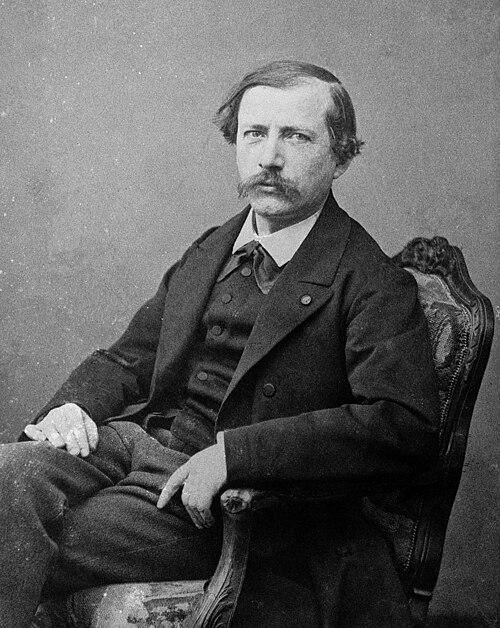
\includegraphics[width=\linewidth]{images/book3/berthelot.jpg}
\end{minipage}\hfill
\begin{minipage}[t]{0.76\linewidth}\vspace{0pt}
Marcellin Berthelot (1827--1907) brûla des composés organiques dans du
dioxygène comprimé, à l'intérieur d'une enceinte close en acier doublée de platine, de sorte que la
combustion était complète et que rien ne s'échappait~: la bombe calorimétrique, aujourd'hui encore
l'instrument de référence pour les chaleurs de combustion. On lui doit aussi les mots
\omterm{def:b2:reaction-enthalpy:exothermic}{exothermique} et \omterm{def:b2:reaction-enthalpy:exothermic}{endothermique}. (Photographie~: domaine public, Wikimedia
Commons.)
\end{minipage}
\end{history}

\section{Exercices}

\begin{exercise}[$\star$]\label{exo:b2:reaction-enthalpy:1}
À l'aide des \omterm{def:b2:reaction-enthalpy:formation}{enthalpies standard de formation} du chapitre, calculer
$\Delta_r H^\circ$ à \qty{298}{K} pour la combustion du propane,
\ce{C3H8(g) + 5O2(g) -> 3CO2(g) + 4H2O(l)}, sachant que $\Delta_f
H^\circ(\ce{C3H8}, \text{g}) = \qty{-104.7}{kJ/mol}$. La réaction est-elle
\omterm{def:b2:reaction-enthalpy:exothermic}{exothermique}~?
% ledger: dfh:C3H8_g
\end{exercise}

\begin{exercise}[$\star$]\label{exo:b2:reaction-enthalpy:2}
Calculer la chaleur libérée par la combustion de \qty{1.00}{kg} de méthane (eau
formée à l'état liquide) et de \qty{1.00}{kg} de dihydrogène, \ce{H2(g) + 1/2O2(g) ->
H2O(l)}. Quel combustible fournit le plus de chaleur par kilogramme~?
\end{exercise}

\begin{exercise}[$\star$]\label{exo:b2:reaction-enthalpy:3}
Une bombe calorimétrique donne $\Delta_r U = \qty{-3264}{kJ/mol}$ pour la combustion
du benzène liquide selon \ce{C6H6(l) + 15/2O2(g) -> 6CO2(g) + 3H2O(l)} à
\qty{298}{K}. Calculer $\Delta_r H$.
\end{exercise}

\begin{exercise}[$\star$]\label{exo:b2:reaction-enthalpy:4}
Sachant que $\Delta_r H^\circ = \qty{-393.5}{kJ/mol}$ pour \ce{C(s) + O2(g) ->
CO2(g)} et $\Delta_r H^\circ = \qty{-283.0}{kJ/mol}$ pour \ce{CO(g) +
1/2O2(g) -> CO2(g)}, calculer l'enthalpie de \ce{CO2(g) + C(s) -> 2CO(g)},
la réaction qui a lieu dans le coke chaud d'un haut fourneau.
\end{exercise}

\begin{exercise}[$\star\star$]\label{exo:b2:reaction-enthalpy:5}
Estimer, avec les enthalpies de liaison du chapitre, l'enthalpie de
\ce{CH4(g) + Cl2(g) -> CH3Cl(g) + HCl(g)}, en prenant \qty{350}{kJ/mol} pour
C--Cl. Calculer ensuite la même grandeur à partir des enthalpies de formation,
sachant que $\Delta_f H^\circ(\ce{CH3Cl}, \text{g}) = \qty{-83.7}{kJ/mol}$, et
commenter l'écart.
% ledger: dfh:CH3Cl_g
\end{exercise}

\begin{exercise}[$\star\star$]\label{exo:b2:reaction-enthalpy:6}
L'enthalpie standard de vaporisation de l'eau à \qty{298}{K} est
$\Delta_f H^\circ(\ce{H2O}, \text{g}) - \Delta_f H^\circ(\ce{H2O},
\text{l})$. La calculer. Avec $C_{p,m}^\circ = \qty{75.35}{J/(K.mol)}$ pour
le liquide et \qty{33.59}{J/(K.mol)} pour la vapeur, toutes deux supposées
constantes, l'estimer à \qty{400}{K} (eau surchauffée sous pression),
et comparer aux tables, qui donnent $\Delta_f H^\circ =
\qty{-282.59}{kJ/mol}$ pour le liquide et \qty{-242.85}{kJ/mol} pour la
vapeur à \qty{400}{K}.
% ledger: cp:H2O_l.298, cp:H2O_g.298, janafdfH:H2O_l.400, janafdfH:H2O_g.400
\end{exercise}

\begin{exercise}[$\star\star$]\label{exo:b2:reaction-enthalpy:7}
Utiliser un cycle de Born--Haber pour calculer l'\omterm{def:b2:reaction-enthalpy:lattice-enthalpy}{enthalpie réticulaire} du chlorure
de potassium à partir de~: $\Delta_f H^\circ(\ce{KCl}, \text{s}) = \qty{-436.7}{kJ/mol}$,
sublimation du potassium \qty{89.0}{kJ/mol}, énergie d'ionisation du
potassium \qty{4.341}{eV}, $\Delta_f H^\circ(\ce{Cl}, \text{g}) =
\qty{121.3}{kJ/mol}$, affinité électronique du chlore \qty{3.613}{eV}. Pourquoi
est-elle plus petite que celle du chlorure de sodium~?
% ledger: dfh:KCl_cr, dfh:K_g, ie:K, janaf:Cl, ea:Cl
\end{exercise}

\begin{exercise}[$\star\star$]\label{exo:b2:reaction-enthalpy:8}
Un calorimètre à pression constante (un simple gobelet isolé) est étalonné en y dissipant \qty{2.00}{kJ}
d'énergie électrique, ce qui élève sa température de \qty{0.418}{K}. On y mélange ensuite
\qty{50.0}{mL} d'acide chlorhydrique à \qty{1.00}{mol/L}
et \qty{50.0}{mL} de solution d'hydroxyde de sodium à \qty{1.10}{mol/L},
toutes deux à la même température initiale~: la température s'élève de
\qty{0.583}{K}. Calculer l'enthalpie de \ce{H3O+(aq) + OH-(aq) ->
2H2O(l)}.
\end{exercise}

\begin{exercise}[$\star\star$]\label{exo:b2:reaction-enthalpy:9}
L'octane, modèle de l'essence, a pour $\Delta_f H^\circ(\text{l}) =
\qty{-250.3}{kJ/mol}$. Calculer l'enthalpie de sa combustion (eau
liquide), la chaleur libérée par kilogramme et la masse de dioxyde de carbone
émise par mégajoule. Comparer au méthane.
% ledger: dfh:C8H18
\end{exercise}

\begin{exercise}[$\star\star\star$]\label{exo:b2:reaction-enthalpy:10}
Calculer la \omterm{def:b2:reaction-enthalpy:flame-temperature}{température de flamme adiabatique} du méthane brûlant dans la
quantité stœchiométrique de dioxygène pur, avec des capacités thermiques constantes (celles
du chapitre à \qty{298}{K}~: \ce{CO2} 37.13, \ce{H2O(g)}
\qty{33.59}{J/(K.mol)}). Comparer au résultat dans l'air,
\qty{2780}{K} dans la même approximation. Pourquoi la flamme réelle dans le dioxygène est-elle
bien plus froide que ne l'indique ce calcul~?
% ledger: cp:CO2_g.298, cp:H2O_g.298
\end{exercise}

\begin{exercise}[$\star\star\star$]\label{exo:b2:reaction-enthalpy:11}
La capacité thermique d'un gaz s'écrit souvent $C_{p,m}^\circ = a + bT$. Pour
la synthèse de l'ammoniac, prendre $\Delta_r a = \qty{-60.5}{J/(K.mol)}$ et
$\Delta_r b = \qty{0.0540}{J/(K^2.mol)}$ (ajustés sur les tables entre
\qty{300}{K} et \qty{800}{K}). Intégrer la \omterm{thm:b2:reaction-enthalpy:kirchhoff}{loi de Kirchhoff} de
\qty{298}{K} à \qty{700}{K} et comparer à la valeur des tables,
\qty{-105.2}{kJ/mol}, ainsi qu'à l'estimation à $C_p$ constante.
\end{exercise}

\begin{exercise}[$\star\star\star$]\label{exo:b2:reaction-enthalpy:12}
Le monoxyde d'azote se forme dans les moteurs selon \ce{N2(g) + O2(g) -> 2NO(g)}.
Calculer son \omterm{def:b2:reaction-enthalpy:standard-reaction-enthalpy}{enthalpie standard de réaction} à \qty{298}{K}. Montrer que, si
$\Delta_r C_p^\circ$ est petite, la réaction absorbe à peu près la même chaleur à
\qty{2000}{K}~; à l'aide des capacités thermiques des tables à \qty{298}{K}
(\ce{NO} \qty{29.85}{J/(K.mol)}, \ce{N2} 29.12, \ce{O2}
\qty{29.38}{J/(K.mol)}), estimer la variation entre
\qty{298}{K} et \qty{2000}{K}. Expliquer pourquoi une réaction \omterm{def:b2:reaction-enthalpy:exothermic}{endothermique} peut poser
problème précisément dans les flammes les plus chaudes.
% ledger: dfh:NO_g, cp:NO_g.298, cp:N2_g.298, cp:O2_g.298
\end{exercise}

\section{Problème~: la cartouche de gaz de camping}

\begin{problem}[{Problème du week-end --- l'énergie du butane, une mesure dans
une bombe calorimétrique, l'eau chauffée dans une casserole et la température de la
flamme}]
\label{pb:b2:reaction-enthalpy:1}
Un réchaud de camping brûle le butane d'une cartouche qui en contient \qty{230}{g}.
Données à \qty{298}{K} ($\Delta_f H^\circ$ en \unit{kJ/mol})~: \ce{C4H10(g)}
$-125.6$, \ce{CO2(g)} $-393.51$, \ce{H2O(l)} $-285.83$, \ce{H2O(g)}
$-241.83$. Masses molaires~: \ce{C4H10} \qty{58.12}{g/mol}, \ce{H2O}
\qty{18.02}{g/mol}. Capacité thermique de l'eau liquide
\qty{75.35}{J/(K.mol)}. Air sec~: \qty{20.95}{\percent} de \ce{O2},
\qty{78.08}{\percent} de \ce{N2}, \qty{0.93}{\percent} de \ce{Ar} en volume. $R = \qty{8.314}{J/(K.mol)}$.
% ledger: dfh:C4H10_g, dfh:CO2, dfh:H2O-l, dfh:H2O_g, cp:H2O_l.298, air:O2, air:N2, air:Ar

\medskip
\noindent\textbf{Partie I --- Le combustible.}
\begin{enumerate}
  \item Écrire la combustion complète du butane, l'eau étant formée à l'état liquide,
        pour une mole de butane.
  \item Calculer son \omterm{def:b2:reaction-enthalpy:standard-reaction-enthalpy}{enthalpie standard de réaction} à \qty{298}{K}.
  \item La calculer de nouveau avec l'eau formée à l'état de vapeur, et expliquer la
        différence.
  \item Calculer la chaleur libérée par gramme de butane dans chaque cas.
  \item Laquelle des deux valeurs décrit un réchaud de camping, dont l'eau
        quitte la flamme à l'état de vapeur~?
  \item Quelle chaleur la cartouche entière peut-elle libérer sur le réchaud~?
\end{enumerate}

\medskip
\noindent\textbf{Partie II --- Une mesure.}
Un échantillon de \qty{0.500}{g} de butane est brûlé dans une bombe calorimétrique de
capacité thermique \qty{10.00}{kJ/K}~; l'eau formée se condense.
\begin{enumerate}[resume]
  \item Quelle grandeur une bombe calorimétrique mesure-t-elle, et pourquoi~?
  \item Calculer le $\Delta\nu_{\text{gaz}}$ de la réaction de la question 1.
  \item Calculer le $\Delta_r U$ attendu.
  \item Calculer l'élévation de température attendue du calorimètre.
  \item L'élévation lue est de \qty{2.461}{K}. En déduire les $\Delta_r U$
        et $\Delta_r H$ mesurés, et l'écart relatif aux tables.
\end{enumerate}

\medskip
\noindent\textbf{Partie III --- La casserole.}
\begin{enumerate}[resume]
  \item Calculer la chaleur nécessaire pour porter \qty{1.00}{L} d'eau
        (\qty{1.00}{kg}) de \qty{20}{\celsius} à \qty{100}{\celsius}.
  \item Le réchaud y parvient avec \qty{16.0}{g} de butane. Calculer son
        rendement (chaleur reçue par l'eau sur chaleur libérée).
  \item Où passe le reste de la chaleur~?
  \item Combien de litres d'eau la cartouche entière peut-elle porter à ébullition
        avec ce rendement~?
\end{enumerate}

\medskip
\noindent\textbf{Partie IV --- La flamme.}
\begin{enumerate}[resume]
  \item Le butane brûle dans la quantité stœchiométrique d'air. Calculer les
        quantités de diazote et d'argon qui accompagnent le dioxygène nécessaire
        à une mole de butane.
  \item Dresser la liste des quantités de produits, diazote et argon compris.
  \item Expliquer, à l'aide d'un chemin en deux étapes, pourquoi la chaleur libérée à
        \qty{298}{K} par la réaction (eau à l'état de vapeur) sert entièrement à
        chauffer ces gaz.
  \item À l'aide des capacités thermiques à \qty{298}{K}, \ce{CO2} 37.13,
        \ce{H2O(g)} 33.59, \ce{N2} 29.12, \ce{Ar} \qty{20.79}{J/(K.mol)},
        calculer la capacité thermique des produits.
  \item En déduire la température de flamme avec des capacités thermiques constantes.
  \item Les incréments d'enthalpie des tables donnent, pour les produits d'une
        mole de butane, \qty{2515.7}{kJ} entre \qty{298}{K} et
        \qty{2300}{K}, et \qty{2655.7}{kJ} entre \qty{298}{K} et
        \qty{2400}{K}. Trouver la température de flamme par interpolation linéaire.
  \item Pourquoi la première estimation est-elle trop élevée~?
  \item Pourquoi la température mesurée d'une flamme de butane est-elle plus basse encore~?
  \item Donner la \omterm{def:b2:reaction-enthalpy:flame-temperature}{température de flamme adiabatique} du butane dans l'air.
\end{enumerate}
\end{problem}
